\documentclass[]{book}
\usepackage{lmodern}
\usepackage{amssymb,amsmath}
\usepackage{ifxetex,ifluatex}
\usepackage{fixltx2e} % provides \textsubscript
\ifnum 0\ifxetex 1\fi\ifluatex 1\fi=0 % if pdftex
  \usepackage[T1]{fontenc}
  \usepackage[utf8]{inputenc}
\else % if luatex or xelatex
  \ifxetex
    \usepackage{mathspec}
  \else
    \usepackage{fontspec}
  \fi
  \defaultfontfeatures{Ligatures=TeX,Scale=MatchLowercase}
\fi
% use upquote if available, for straight quotes in verbatim environments
\IfFileExists{upquote.sty}{\usepackage{upquote}}{}
% use microtype if available
\IfFileExists{microtype.sty}{%
\usepackage{microtype}
\UseMicrotypeSet[protrusion]{basicmath} % disable protrusion for tt fonts
}{}
\usepackage[margin=1in]{geometry}
\usepackage{hyperref}
\hypersetup{unicode=true,
            pdftitle={Abschlussarbeit in RStudio mit Bookdown - A Minimal Tech Example},
            pdfauthor={Felix Kretschmer},
            pdfborder={0 0 0},
            breaklinks=true}
\urlstyle{same}  % don't use monospace font for urls
\usepackage{natbib}
\bibliographystyle{apalike}
\usepackage{color}
\usepackage{fancyvrb}
\newcommand{\VerbBar}{|}
\newcommand{\VERB}{\Verb[commandchars=\\\{\}]}
\DefineVerbatimEnvironment{Highlighting}{Verbatim}{commandchars=\\\{\}}
% Add ',fontsize=\small' for more characters per line
\usepackage{framed}
\definecolor{shadecolor}{RGB}{248,248,248}
\newenvironment{Shaded}{\begin{snugshade}}{\end{snugshade}}
\newcommand{\KeywordTok}[1]{\textcolor[rgb]{0.13,0.29,0.53}{\textbf{{#1}}}}
\newcommand{\DataTypeTok}[1]{\textcolor[rgb]{0.13,0.29,0.53}{{#1}}}
\newcommand{\DecValTok}[1]{\textcolor[rgb]{0.00,0.00,0.81}{{#1}}}
\newcommand{\BaseNTok}[1]{\textcolor[rgb]{0.00,0.00,0.81}{{#1}}}
\newcommand{\FloatTok}[1]{\textcolor[rgb]{0.00,0.00,0.81}{{#1}}}
\newcommand{\ConstantTok}[1]{\textcolor[rgb]{0.00,0.00,0.00}{{#1}}}
\newcommand{\CharTok}[1]{\textcolor[rgb]{0.31,0.60,0.02}{{#1}}}
\newcommand{\SpecialCharTok}[1]{\textcolor[rgb]{0.00,0.00,0.00}{{#1}}}
\newcommand{\StringTok}[1]{\textcolor[rgb]{0.31,0.60,0.02}{{#1}}}
\newcommand{\VerbatimStringTok}[1]{\textcolor[rgb]{0.31,0.60,0.02}{{#1}}}
\newcommand{\SpecialStringTok}[1]{\textcolor[rgb]{0.31,0.60,0.02}{{#1}}}
\newcommand{\ImportTok}[1]{{#1}}
\newcommand{\CommentTok}[1]{\textcolor[rgb]{0.56,0.35,0.01}{\textit{{#1}}}}
\newcommand{\DocumentationTok}[1]{\textcolor[rgb]{0.56,0.35,0.01}{\textbf{\textit{{#1}}}}}
\newcommand{\AnnotationTok}[1]{\textcolor[rgb]{0.56,0.35,0.01}{\textbf{\textit{{#1}}}}}
\newcommand{\CommentVarTok}[1]{\textcolor[rgb]{0.56,0.35,0.01}{\textbf{\textit{{#1}}}}}
\newcommand{\OtherTok}[1]{\textcolor[rgb]{0.56,0.35,0.01}{{#1}}}
\newcommand{\FunctionTok}[1]{\textcolor[rgb]{0.00,0.00,0.00}{{#1}}}
\newcommand{\VariableTok}[1]{\textcolor[rgb]{0.00,0.00,0.00}{{#1}}}
\newcommand{\ControlFlowTok}[1]{\textcolor[rgb]{0.13,0.29,0.53}{\textbf{{#1}}}}
\newcommand{\OperatorTok}[1]{\textcolor[rgb]{0.81,0.36,0.00}{\textbf{{#1}}}}
\newcommand{\BuiltInTok}[1]{{#1}}
\newcommand{\ExtensionTok}[1]{{#1}}
\newcommand{\PreprocessorTok}[1]{\textcolor[rgb]{0.56,0.35,0.01}{\textit{{#1}}}}
\newcommand{\AttributeTok}[1]{\textcolor[rgb]{0.77,0.63,0.00}{{#1}}}
\newcommand{\RegionMarkerTok}[1]{{#1}}
\newcommand{\InformationTok}[1]{\textcolor[rgb]{0.56,0.35,0.01}{\textbf{\textit{{#1}}}}}
\newcommand{\WarningTok}[1]{\textcolor[rgb]{0.56,0.35,0.01}{\textbf{\textit{{#1}}}}}
\newcommand{\AlertTok}[1]{\textcolor[rgb]{0.94,0.16,0.16}{{#1}}}
\newcommand{\ErrorTok}[1]{\textcolor[rgb]{0.64,0.00,0.00}{\textbf{{#1}}}}
\newcommand{\NormalTok}[1]{{#1}}
\usepackage{longtable,booktabs}
\usepackage{graphicx,grffile}
\makeatletter
\def\maxwidth{\ifdim\Gin@nat@width>\linewidth\linewidth\else\Gin@nat@width\fi}
\def\maxheight{\ifdim\Gin@nat@height>\textheight\textheight\else\Gin@nat@height\fi}
\makeatother
% Scale images if necessary, so that they will not overflow the page
% margins by default, and it is still possible to overwrite the defaults
% using explicit options in \includegraphics[width, height, ...]{}
\setkeys{Gin}{width=\maxwidth,height=\maxheight,keepaspectratio}
\IfFileExists{parskip.sty}{%
\usepackage{parskip}
}{% else
\setlength{\parindent}{0pt}
\setlength{\parskip}{6pt plus 2pt minus 1pt}
}
\setlength{\emergencystretch}{3em}  % prevent overfull lines
\providecommand{\tightlist}{%
  \setlength{\itemsep}{0pt}\setlength{\parskip}{0pt}}
\setcounter{secnumdepth}{5}
% Redefines (sub)paragraphs to behave more like sections
\ifx\paragraph\undefined\else
\let\oldparagraph\paragraph
\renewcommand{\paragraph}[1]{\oldparagraph{#1}\mbox{}}
\fi
\ifx\subparagraph\undefined\else
\let\oldsubparagraph\subparagraph
\renewcommand{\subparagraph}[1]{\oldsubparagraph{#1}\mbox{}}
\fi

%%% Use protect on footnotes to avoid problems with footnotes in titles
\let\rmarkdownfootnote\footnote%
\def\footnote{\protect\rmarkdownfootnote}

%%% Change title format to be more compact
\usepackage{titling}

% Create subtitle command for use in maketitle
\newcommand{\subtitle}[1]{
  \posttitle{
    \begin{center}\large#1\end{center}
    }
}

\setlength{\droptitle}{-2em}
  \title{Abschlussarbeit in RStudio mit Bookdown - A Minimal Tech Example}
  \pretitle{\vspace{\droptitle}\centering\huge}
  \posttitle{\par}
  \author{Felix Kretschmer}
  \preauthor{\centering\large\emph}
  \postauthor{\par}
  \predate{\centering\large\emph}
  \postdate{\par}
  \date{2017-08-03}

%\usepackage[ngerman, english]{babel} % this is needed for umlauts and hyphenation
%------- by Nils
%\usepackage[ngerman]{babel}          % NICHT auskommentiert --> Deutsch
%\usepackage[T1]{fontenc}
%\usepackage{lmodern}
%\usepackage[ansinew]{inputenc}
%\usepackage{apacite}
%-------
\usepackage{booktabs}
\usepackage{amsthm}
\makeatletter
\def\thm@space@setup{
  \thm@preskip=8pt plus 2pt minus 4pt
  \thm@postskip=\thm@preskip
}
\makeatother

% from https://github.com/rstudio/bookdown/blob/master/inst/examples/latex/preamble.tex
\makeatletter
\newenvironment{kframe}{%
\medskip{}
\setlength{\fboxsep}{.8em}
 \def\at@end@of@kframe{}%
 \ifinner\ifhmode%
  \def\at@end@of@kframe{\end{minipage}}%
  \begin{minipage}{\columnwidth}%
 \fi\fi%
 \def\FrameCommand##1{\hskip\@totalleftmargin \hskip-\fboxsep
 \colorbox{shadecolor}{##1}\hskip-\fboxsep
     % There is no \\@totalrightmargin, so:
     \hskip-\linewidth \hskip-\@totalleftmargin \hskip\columnwidth}%
 \MakeFramed {\advance\hsize-\width
   \@totalleftmargin\z@ \linewidth\hsize
   \@setminipage}}%
 {\par\unskip\endMakeFramed%
 \at@end@of@kframe}
\makeatother

\renewenvironment{Shaded}{\begin{kframe}}{\end{kframe}}

\newenvironment{rmdblock}[1]
  {
  \begin{itemize}
  \renewcommand{\labelitemi}{
    \raisebox{-.7\height}[0pt][0pt]{
      {\setkeys{Gin}{width=3em,keepaspectratio}\includegraphics{img/#1}}
    }
  }
  \setlength{\fboxsep}{1em}
  \begin{kframe}
  \item
  }
  {
  \end{kframe}
  \end{itemize}
  }
\newenvironment{rmdnote}
  {\begin{rmdblock}{note}}
  {\end{rmdblock}}
\newenvironment{rmdcaution}
  {\begin{rmdblock}{caution}}
  {\end{rmdblock}}
\newenvironment{rmdimportant}
  {\begin{rmdblock}{important}}
  {\end{rmdblock}}
\newenvironment{rmdtip}
  {\begin{rmdblock}{tip}}
  {\end{rmdblock}}
\newenvironment{rmdwarning}
  {\begin{rmdblock}{warning}}
{\end{rmdblock}}
%

\usepackage{amsthm}
\newtheorem{theorem}{Theorem}[chapter]
\newtheorem{lemma}{Lemma}[chapter]
\theoremstyle{definition}
\newtheorem{definition}{Definition}[chapter]
\newtheorem{corollary}{Corollary}[chapter]
\newtheorem{proposition}{Proposition}[chapter]
\theoremstyle{definition}
\newtheorem{example}{Example}[chapter]
\theoremstyle{remark}
\newtheorem*{remark}{Remark}
\let\BeginKnitrBlock\begin \let\EndKnitrBlock\end
\begin{document}
\maketitle

{
\setcounter{tocdepth}{1}
\tableofcontents
}
\listoftables
\listoffigures
\chapter*{Vorbereitung und Vorwort}\label{vorbereitung-und-vorwort}
\addcontentsline{toc}{chapter}{Vorbereitung und Vorwort}

Become a more efficient scientist and collaborate more easily with
colleagues!\\
I really much appreciate what the RStudio Team and people like
\href{https://yihui.name/}{Yihui Xie} are doing to push reproducible
research and our all effiency working with R. And I would love if this
book makes their accomplishments more accessible for students and every
scientist, who is about to set up her or his next R project.

\begin{center}\rule{0.5\linewidth}{\linethickness}\end{center}

\textbf{Why should I read this book?}

\begin{enumerate}
\def\labelenumi{\arabic{enumi}.}
\tightlist
\item
  \emph{Fully dynamic reports}: You have added some new observations?
  Don't worry! All graphics, tables and values will have changed
  automatically after compiling the thesis again. You won't have to copy
  results from your R console and paste it to your word or presentation
  processing program any longer, since

  \begin{enumerate}
  \def\labelenumii{\alph{enumii}.}
  \tightlist
  \item
    R-Chunks allow you to insert tables and graphics using the R code
    you are familiar.
  \item
    You can use inline R code directly in your thesis text, allowing you
    to have R output in your sentences. Just store a result in a
    variable and let R and Markdown print it's value within a sentence.
  \end{enumerate}
\item
  \emph{Be a good scientist!} You are doing real reproducible research
  as we all should do\footnote{I'd really wish publisher would reward
    this!}.

  \begin{enumerate}
  \def\labelenumii{\alph{enumii}.}
  \tightlist
  \item
    Having a dynamic report means every single result you report is
    traceable, so youre reader could see, where every specific value
    comes from.
  \item
    Everything, even the used R packages, are stored within one folder.
    So you can easily share the project and lastly it should compile
    correctly even some years in the future.
  \item
    \emph{Collaborate}: Since your are manipulating plain text files,
    you can use your favorite version control system (e.g.~your
    University's GitLab) and collaborate easily with colleagues.
  \end{enumerate}
\end{enumerate}

\begin{center}\rule{0.5\linewidth}{\linethickness}\end{center}

\subsection*{Contribute!}\label{contribute}
\addcontentsline{toc}{subsection}{Contribute!}

I put a lot of completely unpaid effort and time (since I'm a student
hardcore procrastinating writing his thesis) into making this book and I
give it to you for free, hoping it will save you a lot of time and make
you a better or at least a more efficient researcher.

I though have on request for you: Everyone whom this book helped I want
to invite to contribute to this project as ideas and resolutions, that
would make this book continously better, come during actual thesis
writing or while coding in R.

Maybe you simply want to say ``Thank you!''. Whether my project saved
you time worth 1,000EUR (because you are of the rare species of a well
paid scientist) or you just grant me an after work beer, I would really
appreciate your donation!\footnote{Depending on the way your are reading
  this, you might visit
  \url{https://kreflix.github.io/thesiswritingUsingRStudioAndBookdown/index.html\#contribute}
  to see how to donate.}

Visit

\begin{center}\rule{0.5\linewidth}{\linethickness}\end{center}

\textbf{Objective}

This book and it's corresponding R project shall become a great starting
point for other student's thesises and scientist's statistical reports.
It shall contain everything you usually need while writing a thesis
(especially in Psychology) out of the box, so you can use/copy this R
project folder whenever you start your next R project. Thoug it shall
still be a minimal project and it shall \emph{not} become another
bookdown or R manual. Ferner und von einer nicht zu unterschätzenden
Schwierigkeit (in Details wie Dezimaltrennzeichen etc.) soll dieses
R-Projekt Abschlussarbeiten auf Deutsch ermöglichen.\\
See \protect\hyperlink{tbd}{To be done} if you want to help, but don't
know where to start.

\begin{center}\rule{0.5\linewidth}{\linethickness}\end{center}

As this book is written in order to prepare writing a thesis in German,
you will be confronted with a mixture of languages.\footnote{Auch mein
  Fließtext ist noch work in progress und ich springe zwischen direkter
  und indirekter Anrede, vllt auch zwischen den Anreden Du und Sie.}
Feel free to translate and optimize this book, so it could become a
great starting point for other student's thesises.

\BeginKnitrBlock{rmdcaution}
\emph{tbd}: Dieses Beispielbuch ist noch nicht voll funktionsfähig.
Manches, was in HTML funktioniert, klappt noch nicht im PDF-Output.
Manches davon ist eine Frage der korrekten LaTeX-Einstellungen, manches
wird von bookdown und/oder pandoc nicht unterstützt. Eine Übersicht
findet ihr unter \protect\hyperlink{tbd}{To Be Done}.
\EndKnitrBlock{rmdcaution}

\section*{Get started}\label{get-started}
\addcontentsline{toc}{section}{Get started}

\begin{center}\rule{0.5\linewidth}{\linethickness}\end{center}

\textbf{\emph{tl;dr:}}

\begin{itemize}
\item
  To open and use this book's project just download it's source files
  from GitHub
  \url{http://statistify.de/thesiswritingUsingRStudioAndBookdown_repo}
  or the \texttt{zip} from the toolbar on top of the book's html-version
  and open the \texttt{.Rproj}-file in RStudio (of course you need R and
  RStudio).
\item
  After successfully installing bookdown (see
  \protect\hyperlink{rstudio-und-packrat}{Rstudio und Packrat}) you
  should find the button ``Build Book'' in the ``Build''-tab in RStudio.
  ``Build Book'' creates the book in all output formats. You can find
  the \texttt{index.html}, \texttt{pdf} etc. in the
  \texttt{docs}-folder.

  \begin{itemize}
  \tightlist
  \item
    For PDF-Output you also need to install LaTeX.
  \end{itemize}
\end{itemize}

\begin{center}\rule{0.5\linewidth}{\linethickness}\end{center}

\textbf{\emph{beta:}}

In theory the only thing you need to do is to download the .zip-folder
of this RProject from my
\href{https://github.com/kreflix/thesiswritingUsingRStudioAndBookdown}{Github
Repository} (or clone or fork it if your familiar with GitHub) and open
the \texttt{.RProject}-file. As the R packages contained in the folder
need to be installed for your machine (see
\protect\hyperlink{rstudio-und-packrat}{RStudio und Packrat} ), opening
the RProject may take a few seconds or actually even some minutes. If
you move or share your own project, it migth be a good idea to delete
the folder \texttt{/packrat/lib/} before starting the RProject on a new
machine in order to have a clean installation of the packages.\\
There is also a zip-file containing the RProject downloadable via the
download button on top of this book, if your reading it online. As I
haven't been implementing a routine creating the latter zip
automatically or figured out how to link to my GitHub repo for now, I
cannot promise that it will be the current version of this project.

\BeginKnitrBlock{rmdimportant}
Direct link to the RProject:\\
\url{https://github.com/kreflix/thesiswritingUsingRStudioAndBookdown/archive/master.zip}\\
Be patient while opening the project the first time. Also you might need
an internet connection. Check R Console for what is happening.
\EndKnitrBlock{rmdimportant}

\textbf{\emph{stable:}}

You have to install the \texttt{bookdown}-package in R or could install
the development versions of \textbf{bookdown} from Github:

\begin{Shaded}
\begin{Highlighting}[]
\KeywordTok{install.packages}\NormalTok{(}\StringTok{"bookdown"}\NormalTok{)}
\KeywordTok{library}\NormalTok{(bookdown)}
\CommentTok{#devtools::install_github("rstudio/bookdown")}
\end{Highlighting}
\end{Shaded}

Remember each Rmd file contains one and only one chapter, and a chapter
is defined by the first-level heading \texttt{\#}.

To compile this example to PDF, you need to install XeLaTeX.

I assume you have already installed R and RStudio and you know how to
install any other package this RProject may need (see
\texttt{\_Auswertungsskript.r}).

\hypertarget{rstudio-und-packrat}{\subsection*{RStudio und
Packrat}\label{rstudio-und-packrat}}
\addcontentsline{toc}{subsection}{RStudio und Packrat}

Wenn du den Projektordner dieses Buches heruntergeladen hast (siehe
\protect\hyperlink{links-und-tipps}{Links und Tipps}), verwendest du
automatisch \href{https://rstudio.github.io/packrat/}{Packrat}, da die
entsprechende Projekt-Option bereits aktiviert ist. Das bedeutet, dass
sich die für dieses Buch verwendeten R-Pakete in einer private library
direkt im Projektordner installieren (somit hat jedes Projekt seine
eigenen Pakete).

Da die Pakete auf jedem Computer neu installiert werden müssen,
beinhaltet der Unterordner \texttt{/packrat} anfangs nur die Infos,
welche Pakete du benötigst (einen sogenannten Snapshot). Der Ordner
\texttt{/src} beinhaltet die package tarballs und sollte der
Versionskontrolle unterliegen, wenn du z.B. Git verwendest, sodass das
Projekt auch langfristig reproduzierbar bleibt, selbst dann, wenn die
Pakete nicht mehr online zur Verfügung stehen. \footnote{\emph{tbd}:
  Packrat lädt in meinem Falle trotz hinterlegter tarballs die Pakete
  aus dem Internet.} Die Pakete werden in den Ordner
\texttt{/packrat/lib} installiert, sodass du bei jedem Umzug des
Projektes auf einen neuen PC diesen Ordner zunächst löschen solltest.\\
Mit den folgenden Packrat-Befehlen installierst du alle benötigten
Pakete auf deinem Computer (aufgrund der dependencies der Pakete ist die
Liste recht lang).

\BeginKnitrBlock{rmdcaution}
Beim erstmaligen Start des Projektes wird R versuchen, Packrat und alle
notwendigen Pakete auf deinem Computer zu installieren. Dies kann einige
Minuten dauern und eine Internetverbindung benötigen. Beobachte
währenddessen die Meldungen in der Console. Sollte es nicht automatisch
klappen, dann installiere Packrat manuell. Nutze anschließend folgende
Befehle, um die Pakete zu installieren oder schaue in
\texttt{\_Auswertungsskript.r}, welche Pakete für dieses Buch geladen
werden müssen.
\EndKnitrBlock{rmdcaution}

\begin{Shaded}
\begin{Highlighting}[]
\CommentTok{#packrat::init()  #Initializes the current working directory as a Packrat project.}
\NormalTok{packrat::}\KeywordTok{status}\NormalTok{()}
\NormalTok{packrat::}\KeywordTok{restore}\NormalTok{()}
\NormalTok{packrat::}\KeywordTok{clean}\NormalTok{() }\CommentTok{#löscht scheinbar nicht benötigte Pakete (erkennt Pakete an library() und require() )}
\NormalTok{packrat::}\KeywordTok{get_opts}\NormalTok{()  }\CommentTok{#aktuelle Packrat-Einstellungen}
\end{Highlighting}
\end{Shaded}

After successfully installing R, RStudio, all R packages and
LaTeX\footnote{How to correctly install and set up LaTeX is another
  chapter, that I can't cover by now, because it is still some sort of a
  mystery for me, why some things work while others don't.} (if you want
to create PDF files), you should find the button ``Build Book'' in the
``Build''-tab in RStudio. ``Build Book'' creates the book in all output
formats. You can find the \texttt{index.html}, \texttt{pdf} etc. in the
\texttt{docs}-folder. - For PDF-Output you also need to install LaTeX.

\hypertarget{links-und-tipps}{\section*{Links und
Tipps}\label{links-und-tipps}}
\addcontentsline{toc}{section}{Links und Tipps}

\begin{itemize}
\item
  Yihui Xie wrote a great book, explaining all you need to know about
  bookdown. (\url{https://bookdown.org/yihui/bookdown/})

  \begin{itemize}
  \tightlist
  \item
    Actually I edited his Minimal Book Example to create this book. See
    his original book here:
    \url{https://bookdown.org/yihui/bookdown-demo/} (or download it from
    \href{https://github.com/rstudio/bookdown-demo}{GitHub}).
  \item
    See how the Bookdown-book works under the hood or to follow Yihui's
    example:
    \url{https://github.com/rstudio/bookdown/tree/master/inst/examples}
  \end{itemize}
\item
  I agree with Sean Kross who says ``getting started with bookdown is
  not yet a totally straightforward process''. Read his
  \href{http://seankross.com/2016/11/17/How-to-Start-a-Bookdown-Book.html}{How
  to Start a Bookdown Book} here!

  \begin{itemize}
  \tightlist
  \item
    Actually he provides a
    \href{http://seankross.com/bookdown-start/diving-in.html}{minimal
    bookdown example} as well, but for some reasons his didn't work for
    me. You can download it from
    \href{https://github.com/seankross/bookdown-start}{GitHub}.
  \end{itemize}
\item
  If you move or share your own project, it migth be a good idea to
  delete the folder \texttt{/packrat/lib/} before starting the RProject
  on a new machine in order to have a clean installation of the
  packages.
\item
  There are some cool addins for RStudio, e. g.

  \begin{itemize}
  \tightlist
  \item
    \texttt{citr} Just install it like any other R-package and then you
    can easily insert citations browsing your bib-file within Rstudio.
  \item
    \texttt{ggThemeAssist} or \texttt{ggedit}
  \item
    Find more \url{https://github.com/daattali/addinslist}
  \end{itemize}
\item
  Annotations: \href{https://web.hypothes.is/}{hypothes.is} lets you
  easily and in collaboration with others (or several supervisors)
  annotate text on any website. Of course PDF annotations,
  (Online-)Word's markups, an HTML comment area (e.g.
  \href{https://disqus.com/}{Disqus}) or Git issues could fit your needs
  as well.
\end{itemize}

\subsection*{Auswertungsskript
ausführen}\label{auswertungsskript-ausfuhren}
\addcontentsline{toc}{subsection}{Auswertungsskript ausführen}

Damit alle Ergebnisse, Grafiken und Variablen vorhanden sind, müssen
erst die Berechnungen in R vorgenommen werden. Theoretisch könnten alle
R-Berechnungn auch in einem R-Chunk im Buch ausgeführt werden. Da das
aber bei langen Skripten sehr unüblich werden kann, habe ich ein
klassischen R-Skript zur Auswertung erstellt, dass vor dem Kompilieren
des Buches (ggf. mit Dummy-Daten) ausgeführt werden muss. Entweder per
Hand oder per Source-Befehl.

\begin{Shaded}
\begin{Highlighting}[]
\KeywordTok{source}\NormalTok{(}\StringTok{'_Auswertungsskript.r'}\NormalTok{)}
\end{Highlighting}
\end{Shaded}

\chapter{Buchbestandteile}\label{components}

In vermutlich jeder Thesis gibt es neben Text mindestens auch
Abbildungen und Tabellen. Wie diese eingefügt werden, sodass am Ende
immernoch jedes Output-Format korrekt dargestellt wird, schauen wir uns
im Folgenden an.

This is a \emph{sample} book written in \textbf{Markdown}. You can use
anything that Pandoc's Markdown supports, e.g., a math equation
\(a^2 + b^2 = c^2\).

Ich versuche, Fußnoten, Links, Listen, Aufzählungen etc. nebenher
beispielhaft mit einfließen zu lassen, ohne konkret darauf
einzugehen.\footnote{Für mehr Details sei noch einmal auf Yihui Xie's
  \href{https://bookdown.org/yihui/bookdown/components.html}{Bookdown-Buch}
  hingewiesen!}

\section{Überschriften, Labels und
Absätze}\label{uberschriften-labels-und-absatze}

You can label chapter and section titles using \texttt{\{\#label\}}
after them, e.g., we can reference Chapter \ref{components}. If you do
not manually label them, there will be automatic labels anyway (always
in lowercase), e.g., Chapter \ref{abbildungen}.

Ein neuer Absatz beginnt, wenn eine Leerzeile in Markdown gelassen
wurde.\\
Soll ein Satz in einer neuen Zeile, aber im selben Absatz beginnen, so
müssen nach dem vorhergehenden Satz mehrere Leerzeichen stehen.

\section{Abbildungen}\label{abbildungen}

Figures and tables with captions will be placed in \texttt{figure} and
\texttt{table} environments, respectively.

\begin{Shaded}
\begin{Highlighting}[]
\KeywordTok{par}\NormalTok{(}\DataTypeTok{mar =} \KeywordTok{c}\NormalTok{(}\DecValTok{4}\NormalTok{, }\DecValTok{4}\NormalTok{, .}\DecValTok{1}\NormalTok{, .}\DecValTok{1}\NormalTok{))}
\KeywordTok{plot}\NormalTok{(pressure, }\DataTypeTok{type =} \StringTok{'b'}\NormalTok{, }\DataTypeTok{pch =} \DecValTok{19}\NormalTok{)}
\end{Highlighting}
\end{Shaded}

\begin{figure}

{\centering 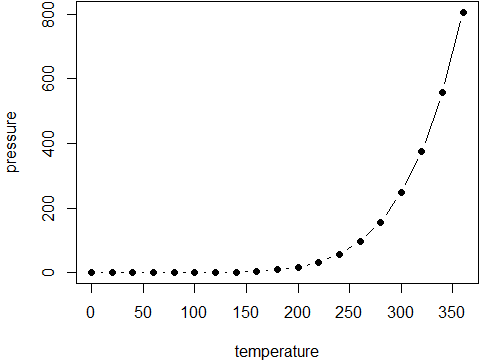
\includegraphics[width=0.8\linewidth]{_main_thesisBookdown_files/figure-latex/nice-fig-1} 

}

\caption{Here is a nice figure!}\label{fig:nice-fig}
\end{figure}

Reference a figure by its code chunk label with the \texttt{fig:}
prefix, e.g., see Figure \ref{fig:nice-fig}.

Externe Grafiken müssen über \texttt{knitr::include\_graphics()}
eingefügt werden, um in PDF, HTML etc. automatisch korrekt referenziert
werden zu können. Fußnoten können überall per
\texttt{\^{}{[}Fußnotentext{]}} eingefügt werden -- so wie hier in der
Bildunterschrift.

\begin{Shaded}
\begin{Highlighting}[]
\NormalTok{knitr::}\KeywordTok{include_graphics}\NormalTok{(}\StringTok{'img/important.png'}\NormalTok{)}
\end{Highlighting}
\end{Shaded}

\textbackslash{}begin\{figure\}

\{\centering 
\includegraphics[width=0.328\linewidth]{img/important}

\}

\textbackslash{}caption\{Zentriertes Bild aus externer
PNG-Datei.\footnote{\url{http://statistify.de}}\}\label{fig:externalImage}
\textbackslash{}end\{figure\}

\section{Tabellen}\label{tabellen}

\subsection{knitr-Tabelle}\label{knitr-tabelle}

Similarly to figures, you can reference tables generated from
\texttt{knitr::kable()}, e.g., see Table \ref{tab:knitrTable}.

\begin{Shaded}
\begin{Highlighting}[]
\NormalTok{knitr::}\KeywordTok{kable}\NormalTok{(}
  \KeywordTok{head}\NormalTok{(iris, }\DecValTok{5}\NormalTok{), }\DataTypeTok{caption =} \StringTok{'This knitr::kable() table looks great in any output format.'}\NormalTok{,}
  \DataTypeTok{booktabs =} \OtherTok{TRUE}
\NormalTok{)}
\end{Highlighting}
\end{Shaded}

\begin{table}

\caption{\label{tab:knitrTable}This knitr::kable() table looks great in any output format.}
\centering
\begin{tabular}[t]{rrrrl}
\toprule
Sepal.Length & Sepal.Width & Petal.Length & Petal.Width & Species\\
\midrule
5.1 & 3.5 & 1.4 & 0.2 & setosa\\
4.9 & 3.0 & 1.4 & 0.2 & setosa\\
4.7 & 3.2 & 1.3 & 0.2 & setosa\\
4.6 & 3.1 & 1.5 & 0.2 & setosa\\
5.0 & 3.6 & 1.4 & 0.2 & setosa\\
\bottomrule
\end{tabular}
\end{table}

\subsection{komplexere (LaTeX-)Tabellen}\label{complexTables}

\texttt{knitr:::kable()} erlaubt leider kein row- oder colspan, also
keine Tabellenzellen, die über mehrere Reihen oder Spalten gehen. Ebenso
gehen Markdown-Tabellen mit Span nicht, da dies in
\href{http://www.pandoc.org/MANUAL.html\#tables}{Pandoc} flavored
markdown nicht unterstützt wird.

\begin{verbatim}
Table: \label{tab:rmdTable} Broken Table.

| One    | Two | Three | Four    | Five  | Six 
| -
| Span <td colspan=3>triple  <td colspan=2>double
\end{verbatim}

Ergibt eine kaputte Tabelle \ref{tab:rmdTable}:

\begin{longtable}[]{@{}l@{}}
\caption{\label{tab:rmdTable}Broken Table.}\tabularnewline
\toprule
One\tabularnewline
\midrule
\endfirsthead
\toprule
One\tabularnewline
\midrule
\endhead
\bottomrule
\end{longtable}

\textbar{} Span

triple

double

Möchte man eine Tabelle ohne \texttt{knitr:::kable()} und ohne Pandoc
erstellen, kann das Buch nicht mehr automatisch in jedes Output-Format
kompiliert werden. Man kann aber selbst die Bedingung schreiben, bei
welchem Output-Format welches Tabellenformat gewählt werden soll.

\begin{Shaded}
\begin{Highlighting}[]
\NormalTok{if( knitr:::}\KeywordTok{is_latex_output}\NormalTok{() ) \{ ... \}}
\end{Highlighting}
\end{Shaded}

Dies kann man nutzen, um zumindest in PDF komplexe LaTeX-Tabellen zu
erzeugen, während in HTML und Co. eine nicht ganz so schöne Tabelle
dargestellt wird. Beachtet die R-Chunk-Optionen
\texttt{results=\textquotesingle{}asis} und
\texttt{comment=\textquotesingle{}\textquotesingle{}} sowie kleine
Syntaxanpassungen im R-Befehl \texttt{cat()} wie
\texttt{\textbackslash{}\textbackslash{}} und
\texttt{\textbackslash{}n}, um in LaTeX kompilierbaren Output aus R
heraus zu generieren.

\begin{verbatim}
{r latexTable, fig.cap='latexTable', results='asis', comment=''}
\end{verbatim}

\begin{Shaded}
\begin{Highlighting}[]
\NormalTok{if( knitr:::}\KeywordTok{is_latex_output}\NormalTok{() ) \{}
  \CommentTok{#erstelle LaTeX-Tabelle über R-Output}
    \CommentTok{#(beachte die Syntaxanpassung "cat()", "\textbackslash{}\textbackslash{}" und "\textbackslash{}n", um LaTeX-Output aus R zu erzeugen):}
    \KeywordTok{cat}\NormalTok{(}\StringTok{"}\CharTok{\textbackslash{}\textbackslash{}}\StringTok{begin\{table\}[]}\CharTok{\textbackslash{}n}\StringTok{"}\NormalTok{)}
    \KeywordTok{cat}\NormalTok{(}\StringTok{"}\CharTok{\textbackslash{}\textbackslash{}}\StringTok{centering}\CharTok{\textbackslash{}n}\StringTok{"}\NormalTok{)}
    \KeywordTok{cat}\NormalTok{(}\StringTok{"}\CharTok{\textbackslash{}\textbackslash{}}\StringTok{caption\{(}\CharTok{\textbackslash{}\textbackslash{}}\StringTok{#tab:latexTable) Pure LaTeX-Table\}}\CharTok{\textbackslash{}n}\StringTok{"}\NormalTok{)}
    \KeywordTok{cat}\NormalTok{(}\StringTok{"}\CharTok{\textbackslash{}\textbackslash{}}\StringTok{label\{latexTable\}}\CharTok{\textbackslash{}n}\StringTok{"}\NormalTok{)}
    \KeywordTok{cat}\NormalTok{(}\StringTok{"}\CharTok{\textbackslash{}\textbackslash{}}\StringTok{begin\{tabular\}\{lllll\}}\CharTok{\textbackslash{}n}\StringTok{"}\NormalTok{)}
    \KeywordTok{cat}\NormalTok{(}\StringTok{"            & }\CharTok{\textbackslash{}\textbackslash{}}\StringTok{textbf\{c1\}  & }\CharTok{\textbackslash{}\textbackslash{}}\StringTok{textbf\{c2\} & }\CharTok{\textbackslash{}\textbackslash{}}\StringTok{textbf\{c3\}  & }\CharTok{\textbackslash{}\textbackslash{}}\StringTok{textbf\{c4\} }\CharTok{\textbackslash{}\textbackslash{}\textbackslash{}\textbackslash{}\textbackslash{}n}\StringTok{"}\NormalTok{)}
    \KeywordTok{cat}\NormalTok{(}\StringTok{"}\CharTok{\textbackslash{}\textbackslash{}}\StringTok{textit\{r1\} & }\CharTok{\textbackslash{}\textbackslash{}}\StringTok{multicolumn\{2\}\{c\}\{r1c1c2\} & r1c3         & r1c4        }\CharTok{\textbackslash{}\textbackslash{}\textbackslash{}\textbackslash{}\textbackslash{}n}\StringTok{"}\NormalTok{)}
    \KeywordTok{cat}\NormalTok{(}\StringTok{"}\CharTok{\textbackslash{}\textbackslash{}}\StringTok{textit\{r2\} & r2c1         & r2c2        & }\CharTok{\textbackslash{}\textbackslash{}}\StringTok{multicolumn\{2\}\{c\}\{r2c3c4\}}\CharTok{\textbackslash{}n}\StringTok{"}\NormalTok{)}
    \KeywordTok{cat}\NormalTok{(}\StringTok{"}\CharTok{\textbackslash{}\textbackslash{}}\StringTok{end\{tabular\}}\CharTok{\textbackslash{}n}\StringTok{"}\NormalTok{)}
    \KeywordTok{cat}\NormalTok{(}\StringTok{"}\CharTok{\textbackslash{}\textbackslash{}}\StringTok{end\{table\}}\CharTok{\textbackslash{}n}\StringTok{"}\NormalTok{)}
    
    \CommentTok{#erzeugt folgenden in LaTeX kompilierbaren Output:}
    \CommentTok{# \textbackslash{}begin\{table\}[]}
    \CommentTok{# \textbackslash{}centering}
    \CommentTok{# \textbackslash{}caption\{caption="(\textbackslash{}\textbackslash{}#tab:xTable) An xtable table")Pure LaTeX-Table\}}
    \CommentTok{# \textbackslash{}label\{latexTable\}}
    \CommentTok{# \textbackslash{}begin\{tabular\}\{lllll\}}
    \CommentTok{#             & \textbackslash{}textbf\{c1\}  & \textbackslash{}textbf\{c2\} & \textbackslash{}textbf\{c3\}  & \textbackslash{}textbf\{c4\} \textbackslash{}\textbackslash{}}
    \CommentTok{# \textbackslash{}textit\{r1\} & \textbackslash{}multicolumn\{2\}\{c\}\{r1c1c2\} & r1c3         & r1c4        \textbackslash{}\textbackslash{}}
    \CommentTok{# \textbackslash{}textit\{r2\} & r2c1         & r2c2        & \textbackslash{}multicolumn\{2\}\{c\}\{r2c3c4\}}
    \CommentTok{# \textbackslash{}end\{tabular\}}
    \CommentTok{# \textbackslash{}end\{table\}}
\NormalTok{\} else \{}
  \CommentTok{#erstelle Tabelle für alle anderen Outputformate:}
    \NormalTok{rcMatrix <-}\StringTok{ }\KeywordTok{t}\NormalTok{(}\KeywordTok{data.frame}\NormalTok{(}\KeywordTok{c}\NormalTok{(}\StringTok{"r1c1c2"}\NormalTok{, }\StringTok{""}\NormalTok{, }\StringTok{"r1c3"}\NormalTok{, }\StringTok{"r1c4"}\NormalTok{),}
                             \KeywordTok{c}\NormalTok{(}\StringTok{"r2c1"}\NormalTok{, }\StringTok{"r2c2"}\NormalTok{, }\StringTok{""}\NormalTok{, }\StringTok{"r2c3c4"}\NormalTok{) ))}
      \KeywordTok{colnames}\NormalTok{(rcMatrix) <-}\StringTok{ }\KeywordTok{c}\NormalTok{(}\StringTok{"c1"}\NormalTok{, }\StringTok{"c2"}\NormalTok{, }\StringTok{"c3"}\NormalTok{, }\StringTok{"c4"}\NormalTok{)}
      \KeywordTok{rownames}\NormalTok{(rcMatrix) <-}\StringTok{ }\KeywordTok{c}\NormalTok{(}\StringTok{"r1"}\NormalTok{, }\StringTok{"r2"}\NormalTok{)}
    
    \NormalTok{knitr::}\KeywordTok{kable}\NormalTok{(}
      \NormalTok{rcMatrix, }\DataTypeTok{caption =} \StringTok{'This table would be a pure LaTeX table with proper colspan in PDF'}\NormalTok{,}
      \DataTypeTok{booktabs =} \OtherTok{TRUE}
    \NormalTok{)}
\NormalTok{\}}
\end{Highlighting}
\end{Shaded}

\begin{table}[]
\centering
\caption{\label{tab:latexTable} Pure LaTeX-Table}
\label{latexTable}
\begin{tabular}{lllll}
            & \textbf{c1}  & \textbf{c2} & \textbf{c3}  & \textbf{c4} \\
\textit{r1} & \multicolumn{2}{c}{r1c1c2} & r1c3         & r1c4        \\
\textit{r2} & r2c1         & r2c2        & \multicolumn{2}{c}{r2c3c4}
\end{tabular}
\end{table}

As \href{https://bookdown.org/yihui/bookdown/tables.html}{Yihui}
mentions ``{[}if{]} you decide to use other R packages to generate
tables, you have to make sure the label for the table environment
appears in the beginning of the table caption in the form
\texttt{(\textbackslash{}\#label)} (again, label must have the prefix
tab:):''\\
Since \texttt{\textbackslash{}} (backslash) is an escape sequence, we
have to write
\texttt{(\textbackslash{}\textbackslash{}\#tab:Beschriftung)} here.

Da der R-Chunk die Option
\texttt{fig.cap=\textquotesingle{}latexTable\textquotesingle{}}
beinhaltet und der Tabellenüberschrifts-LaTeX-Befehl
\texttt{(\textbackslash{}\textbackslash{}\#tab:latexTable))} enthält,
kann man in beiden Output-Bedingungen per
\texttt{\textbackslash{}@ref(tab:latexTable)} auf die Tabelle
referenzieren: Siehe Tabelle \ref{tab:latexTable}.

\subsection{xTable()}\label{xTable}

Ein beliebtes R-package zur Erstellung von LaTeX-Tabellen ist
\texttt{xtable}. Auch wenn Tabelle \ref{tab:xTable} aussieht wie jede
anderen, wurde sie mit xtable erstellt.\\
xtable unterstützt nur die Outputformate PDF (default) und HTML
(\texttt{type=\textquotesingle{}html\textquotesingle{}}), die aber nicht
automatisch je nach gewähltem Outputformat ausgegeben werden. So muss,
wie schon in Abschnitt \ref{complexTables} gezeigt, für jede
Output-Bedingung eine eigene Tabelle erstellt werden.\\
Die R-Chunk-Option
\texttt{results=\textquotesingle{}asis\textquotesingle{}} sowie
\texttt{print.xtable(...,\ comment=FALSE)} sorgen dafür, dass der
R-Output in LaTeX kompilierbar ist.

\begin{verbatim}
{r xTable, fig.cap='xTable', echo=TRUE, results='asis'}
\end{verbatim}

\begin{Shaded}
\begin{Highlighting}[]
\NormalTok{if( knitr:::}\KeywordTok{is_latex_output}\NormalTok{() ) \{}
  \CommentTok{#PDF}
  \KeywordTok{library}\NormalTok{(xtable)}
  \KeywordTok{print.xtable}\NormalTok{(}
    \KeywordTok{xtable}\NormalTok{(mtcars[}\DecValTok{1}\NormalTok{:}\DecValTok{3}\NormalTok{,}\DecValTok{1}\NormalTok{:}\DecValTok{4}\NormalTok{], }\DataTypeTok{label=}\StringTok{"xTableInternLabel"}\NormalTok{, }\DataTypeTok{caption=}\StringTok{"(}\CharTok{\textbackslash{}\textbackslash{}}\StringTok{#tab:xTable) An xtable table"}\NormalTok{), }\DataTypeTok{comment=}\OtherTok{FALSE}\NormalTok{)}
\NormalTok{\} else if ( knitr:::}\KeywordTok{is_html_output}\NormalTok{() ) \{}
  \CommentTok{#HTML}
  \KeywordTok{library}\NormalTok{(xtable)}
  \KeywordTok{print.xtable}\NormalTok{(}
    \KeywordTok{xtable}\NormalTok{(mtcars[}\DecValTok{1}\NormalTok{:}\DecValTok{3}\NormalTok{,}\DecValTok{1}\NormalTok{:}\DecValTok{4}\NormalTok{], }\DataTypeTok{label=}\StringTok{"xTableInternLabel"}\NormalTok{, }\DataTypeTok{caption=}\StringTok{"(}\CharTok{\textbackslash{}\textbackslash{}}\StringTok{#tab:xTable) An xtable table"}\NormalTok{), }\DataTypeTok{comment=}\OtherTok{FALSE}\NormalTok{,}
    \DataTypeTok{type=}\StringTok{'html'}\NormalTok{) }\CommentTok{#only 'latex' (default) or 'html'}
\NormalTok{\} else \{}
  \CommentTok{#Word und andere Outputformate  }
  \NormalTok{knitr::}\KeywordTok{kable}\NormalTok{(}
    \NormalTok{mtcars[}\DecValTok{1}\NormalTok{:}\DecValTok{3}\NormalTok{,}\DecValTok{1}\NormalTok{:}\DecValTok{4}\NormalTok{], }\DataTypeTok{caption =} \StringTok{'In other output formats than PDF and HTML we cannot use xtable'}\NormalTok{,}
    \DataTypeTok{booktabs =} \OtherTok{TRUE}
    \NormalTok{)}
\NormalTok{\}}
\end{Highlighting}
\end{Shaded}

\begin{table}[ht]
\centering
\begin{tabular}{rrrrr}
  \hline
 & mpg & cyl & disp & hp \\ 
  \hline
Mazda RX4 & 21.00 & 6.00 & 160.00 & 110.00 \\ 
  Mazda RX4 Wag & 21.00 & 6.00 & 160.00 & 110.00 \\ 
  Datsun 710 & 22.80 & 4.00 & 108.00 & 93.00 \\ 
   \hline
\end{tabular}
\caption{\label{tab:xTable} An xtable table} 
\label{xTableInternLabel}
\end{table}

\BeginKnitrBlock{rmdcaution}
Only HTML and PDF are supported output formats in xtable().
\EndKnitrBlock{rmdcaution}

\subsection{interaktive Tabellen}\label{interactiveTable}

Es können auch interaktive Tabellen eingefügt werden. Diese ergeben
natürlich in statischen Dokumenten wie PDF keinen Sinn. In PDF kann aber
ein \textbf{Screenshot} der dynamischen Tabelle/Abbildung automatisch
eingefügt werden.

Problematisch beim Erstellen von Tabellen mit anderen Paketen ist die
korrekte \emph{Tabellennummerierung}! HTML-Widgets sind meistens Plots,
weswegen Yihui vorerst auch die \texttt{DT}-Widgets nur als
``Abbildung'' bezeichnen und nummerieren lassen wird. Siehe
\href{https://github.com/rstudio/bookdown/issues/313}{issue 313} auf
GitHub.\\
Um immerhin die Nummerierung als Abbild hinzubekommen, benötigt der
R-Code-Chunk, der die Tabelle(ngrafik) erstellt, die Option
\texttt{fig.cap}. Für einen schönen Screenshot gibt es etliche
Chunk-Options via \texttt{screenshot.opts}.

\begin{verbatim}
{r dynamicTableWebshot, fig.cap='dynamicTableWebshot', dev='png', cache=TRUE, cache.extra=packageVersion('DT'), screenshot.opts=list(zoom=2)}
\end{verbatim}

\begin{Shaded}
\begin{Highlighting}[]
  \CommentTok{#library(webshot)}
  \CommentTok{#webshot::install_phantomjs()  #muss für Screenshot installiert werden}
  \NormalTok{DT::}\KeywordTok{datatable}\NormalTok{(}
    \KeywordTok{head}\NormalTok{(iris, }\DecValTok{20}\NormalTok{), }\DataTypeTok{caption =} \StringTok{'This table is a screenshot in PDF, but interactive in HTML.'}\NormalTok{)}
\end{Highlighting}
\end{Shaded}

\begin{figure}[htbp]
\centering
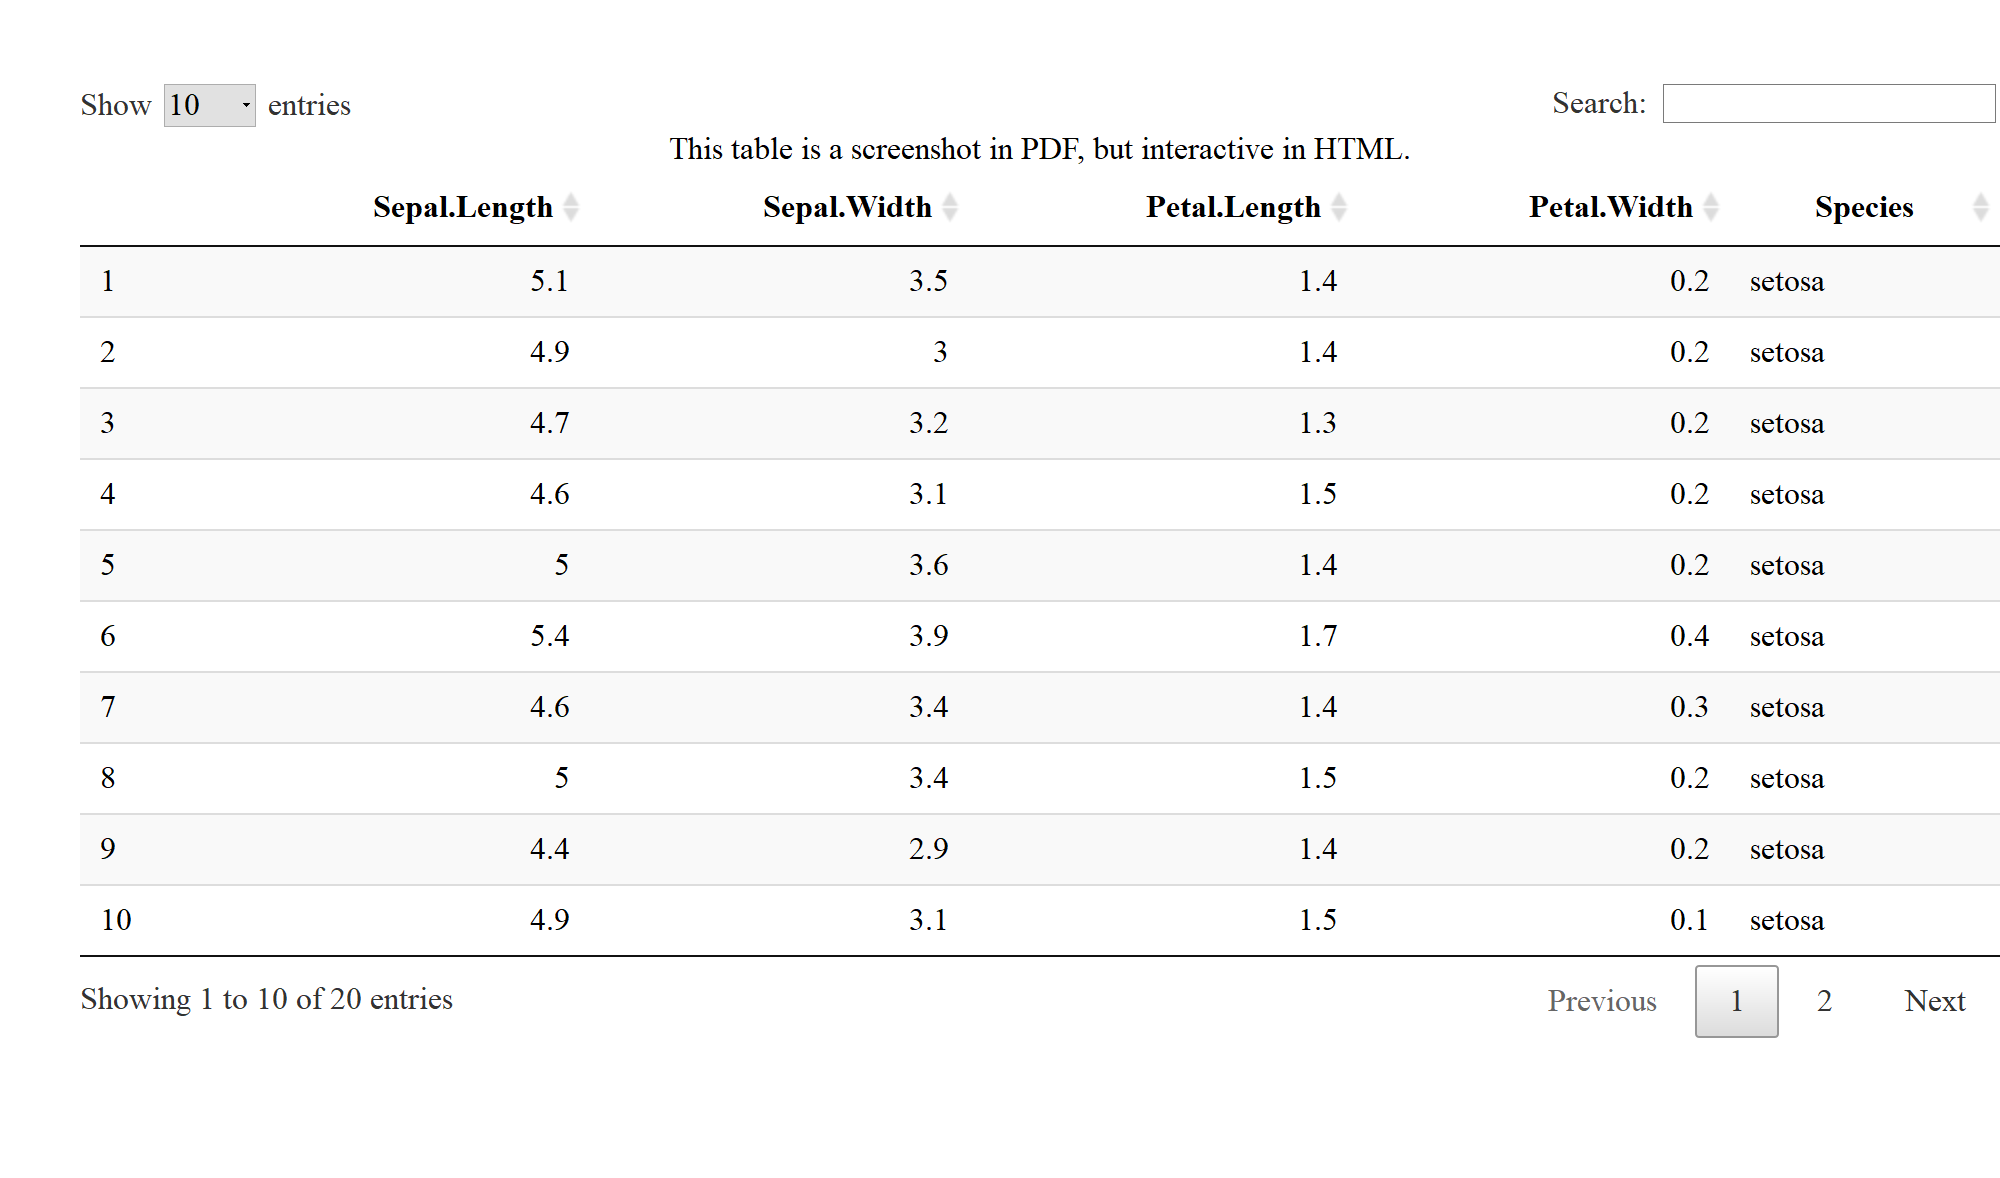
\includegraphics{_main_thesisBookdown_files/figure-latex/dynamicTableWebshot-1.png}
\caption{\label{fig:dynamicTableWebshot}dynamicTableWebshot}
\end{figure}

\begin{verbatim}
1. See Table \\ref{tab:dynamicTableWebshot} (Tabellenreferenz-Syntax)
1. See Table \\ref{fig:dynamicTableWebshot} (Abbildungsreferenz-Syntax)
1. See Table \\ref{dynamicTableWebshot} (Überschriftsreferenz-Syntax)
\end{verbatim}

\begin{enumerate}
\def\labelenumi{\arabic{enumi}.}
\tightlist
\item
  See Table \ref{tab:dynamicTableWebshot} (Tabellenreferenz-Syntax)
\item
  See Table \ref{fig:dynamicTableWebshot} (Abbildungsreferenz-Syntax)
\item
  See Table \ref{dynamicTableWebshot} (Überschriftsreferenz-Syntax)
\end{enumerate}

\BeginKnitrBlock{rmdcaution}
HTML-Widgets, müssen als \textbf{Abbildung}
(\texttt{\textbackslash{}@ref(fig:BeschriftungstextFigCap}) referenziert
werden, auch wenn es sich um eine DT-Tabelle handelt.
\EndKnitrBlock{rmdcaution}

\subsection{Inline R-Code}\label{inline-r-code}

\subsubsection{Referenzieren mit
Inline-Bedingung}\label{referenzieren-mit-inline-bedingung}

\emph{Kann ich nicht je nach Outputformat eine statische oder
interaktive Tabelle erzeugen?}

Leider kann das Vorgehen wie unter Abschnitt \ref{complexTables}
beschrieben für DT-Tabellen (HTML-Widget) nicht empfohlen werden. Da in
HTML die interaktive htmlwidget-Tabelle als Abbildung aufgefasst wird,
aber als Tabelle in PDF, ergeben sich unterschiedliche Nummerierungen in
HTML und PDF. Zwar sind die Nummerierungen innerhalb eines Dokuments
konsistent, aber man muss stets darauf achten, ob man die Tabelle mit
\texttt{\textbackslash{}@ref(tab:Tabellenbezeichnung)} (HTML) oder mit
\texttt{\textbackslash{}@ref(fig:Tabellenbezeichnung)} (PDF)
referenziert.

\BeginKnitrBlock{rmdimportant}
HTML-Widgets werden auch dann als Abbildung geführt, wenn es sich um
eine DT-Tabelle handelt.
\EndKnitrBlock{rmdimportant}

Wie referenziere ich nun auf die Tabelle, wenn sie einmal eine Tabelle
und einmal eine Abbildung ist? Probieren wir es anhand der folgenden
Tabelle aus.

\begin{Shaded}
\begin{Highlighting}[]
\NormalTok{if( knitr:::}\KeywordTok{is_html_output}\NormalTok{() ) \{}
  \CommentTok{#interactives HTML-Widget}
  \CommentTok{#library(webshot)}
  \CommentTok{#webshot::install_phantomjs()  #muss für Screenshot installiert werden}
  \NormalTok{DT::}\KeywordTok{datatable}\NormalTok{(}
    \NormalTok{mtcars[}\DecValTok{1}\NormalTok{:}\DecValTok{3}\NormalTok{,}\DecValTok{1}\NormalTok{:}\DecValTok{4}\NormalTok{], }\DataTypeTok{caption =} \StringTok{'This table is a screenshot in PDF, but interactive in HTML.'}\NormalTok{)}
\NormalTok{\} else \{}
  \CommentTok{#statische Tabelle in allen anderen Outputformaten  }
  \NormalTok{knitr::}\KeywordTok{kable}\NormalTok{(}
    \NormalTok{mtcars[}\DecValTok{1}\NormalTok{:}\DecValTok{3}\NormalTok{,}\DecValTok{1}\NormalTok{:}\DecValTok{4}\NormalTok{], }\DataTypeTok{caption =} \StringTok{'This table would be interactive in HTML.'}\NormalTok{,}
    \DataTypeTok{booktabs =} \OtherTok{TRUE}
    \NormalTok{)}
\NormalTok{\}}
\end{Highlighting}
\end{Shaded}

\begin{table}

\caption{\label{tab:htmlWidgetTableCondition}This table would be interactive in HTML.}
\centering
\begin{tabular}[t]{lrrrr}
\toprule
  & mpg & cyl & disp & hp\\
\midrule
Mazda RX4 & 21.0 & 6 & 160 & 110\\
Mazda RX4 Wag & 21.0 & 6 & 160 & 110\\
Datsun 710 & 22.8 & 4 & 108 & 93\\
\bottomrule
\end{tabular}
\end{table}

Folgende Markdown-Textschnipsel ergeben zum Teil unterschiedlichen Text
in PDF und HTML.

\begin{verbatim}
1. See Table \\ref{tab:htmlWidgetTableCondition} will work in PDF, but not in HTML.
1. See Table \\ref{fig:htmlWidgetTableCondition} will work in HTML (and Word btw.), but not in PDF.
1. See Table \\ref{htmlWidgetTableCondition} is just not correct here.
1. See Table `r ifelse ( knitr:::is_html_output(), '\\\ref{fig:htmlWidgetTableCondition}', '\\\ref{tab:htmlWidgetTableCondition}' )` will work in any Output, but is a bit monstrous.
\end{verbatim}

\begin{enumerate}
\def\labelenumi{\arabic{enumi}.}
\tightlist
\item
  See Table \ref{tab:htmlWidgetTableCondition} will work in PDF, but not
  in HTML.
\item
  See Table \ref{fig:htmlWidgetTableCondition} will work in HTML (and
  Word btw.), but not in PDF.
\item
  See Table \ref{htmlWidgetTableCondition} is just not correct here.
\item
  See Table \ref{tab:htmlWidgetTableCondition} will work in any Output,
  but is a bit monstrous.
\end{enumerate}

\subsubsection{Inline R-Output und bedingte
Textanzeige}\label{inline-r-output-und-bedingte-textanzeige}

Letztlich können wir mithilfe von Inline-R-Code auf jede R-Variable
zurückgreifen und überall bedingte Textbausteine in die Thesis einfügen,
was vor allem beim Report statistische Analysen sehr nütztlich ist.

\begin{Shaded}
\begin{Highlighting}[]
\NormalTok{Fahrzeuge mit Automatikgetriebe haben }
\BaseNTok{`r if (t.test(gear~am, data=mtcars)$p.value > 0.05) 'nicht'`} 
\NormalTok{signifikant mehr oder weniger Gänge als Autos mit manuellem Schaltgetriebe.}
\end{Highlighting}
\end{Shaded}

Fahrzeuge mit Automatikgetriebe haben signifikant mehr oder weniger
Gänge als Autos mit manuellem Schaltgetriebe.\\
Im Schnitt haben alle Autos des \texttt{mtcars}-Datensatzes
\texttt{mean(mtcars\$hp)=} 146.6875PS.

\BeginKnitrBlock{rmdimportant}
Mithilfe von Inline-R-Code \texttt{`r\ R-Code`} können wir auf jede
R-Variable und gewohnte R-Funktionalitäten wie bedingte Textanzeigen
zurückgreifen.
\EndKnitrBlock{rmdimportant}

\chapter{Verfassen}\label{verfassen}

Neben Überschriften, Abbildungen und Co. besteht eine Thesis nun mal
hauptsächlich aus Text.\\
Leider unterstützen in einigen Punkten andere Editoren den Schreiber
etwas besser. Microsoft Word hat eine gute as-you-type Rechtschreibung-
und Grammatik-Prüfung inkl. Synonymfunktion. U.a. beim Atom-Editor
scheint man eine Autocompletion nicht nur für Variablen, sondern auch
für Referenzschlüssel (bibtexkeys) aus der \texttt{.bib}-Literaturliste
zu haben. Im Folgenden wollen wir uns Kleinigkeiten anschauen, die uns
das Schreiben und Argumentieren in RStudio erleichtern.

\section{Zitationen}\label{zitationen}

You can write citations, too. For example, we are using the
\textbf{bookdown} package \citep{R-bookdown} in this sample book, which
was built on top of R Markdown and \textbf{knitr} \citep{xie2015}.

Um die genutzten R-Pakete zu zitieren, kann wie folgt eine bib-Datei
erstellt werden, die als bibliography ausgegeben werden kann:

\begin{Shaded}
\begin{Highlighting}[]
\CommentTok{# automatically create a bib database for R packages}
\NormalTok{knitr::}\KeywordTok{write_bib}\NormalTok{(}\KeywordTok{c}\NormalTok{(}
  \KeywordTok{.packages}\NormalTok{(), }\StringTok{'bookdown'}\NormalTok{, }\StringTok{'knitr'}\NormalTok{, }\StringTok{'rmarkdown'}
\NormalTok{), }\StringTok{'packages.bib'}\NormalTok{)}
\end{Highlighting}
\end{Shaded}

Mit dem RStudio Addin \texttt{citr} lässt sich, möchte man einen Autor
zitieren, der passende bibtexkey per Klick heraussuchen. Dabei
durchsucht \texttt{citr} die im YAML-Bereich der \texttt{index.Rmd}
angegebenen bibliography-files (siehe \texttt{.bib}-Dateien im
Projektordner).

\begin{Shaded}
\begin{Highlighting}[]
\CommentTok{#install.packages("citr")}
\KeywordTok{library}\NormalTok{(citr)}
\end{Highlighting}
\end{Shaded}

\begin{itemize}
\tightlist
\item
  \texttt{{[}@xie2015{]}} ergibt: \ldots{} \citep{xie2015} \ldots{}
\item
  \texttt{Xie\ {[}-xie2015{]}} ergibt: \ldots{} Xie
  \citeyearpar{xie2015} \ldots{}
\item
  \texttt{@xie2015} ergibt: \ldots{} \citet{xie2015} \ldots{}
\end{itemize}

Der Zitationsstil übernimmt auch, wenn Autoren das erste Mal anders
zitiert werden sollen \citep{Cole2012} als beim zweiten Mal
\citep{Cole2012}, was bei mehreren Autoren üblich ist.

Und man kann mehrere Autoren gleichzeitig zitieren.\\
\texttt{{[}Vergleiche\ @xie2015,\ Kapitel\ 1;\ und\ auch\ @Cole2012,\ S.\ 33-35\ und\ 41{]}}
ergibt: \ldots{} \citetext{\citealp[Vergleiche][Kapitel
1]{xie2015}; \citealp[und auch][S. 33-35 und 41]{Cole2012}} \ldots{}

\section{Text wiederholen und
Blockquote}\label{text-wiederholen-und-blockquote}

Man kann ganze Textabschnitte wiederholen. Für dieses Beispiel habe ich
mich selbst in einem block qoute zitiert, ohne den Text noch einmal
tippen zu müssen.

\begin{verbatim}


Wie ich vorher schon schrieb:

> Zu wiederholender Text.
>
> --- me
\end{verbatim}

Zu wiederholender Text. Zu wiederholender Text.

Wie ich vorher schon schrieb:

\begin{quote}
Zu wiederholender Text.

--- me
\end{quote}

\section{Spracheinstellungen}\label{spracheinstellungen}

In HTML werden die Tabellen korrekt nummeriert und auch die Übersetzung
(``Abbildung'' statt ``Figure'') kann über die \texttt{\_bookdown.yml}
eingestellt werden. \emph{tbd:} Der Output in LaTeX stimmt leider noch
nicht.

\section{Spell Check}\label{spell-check}

RStudio nutzt die Hunspell Rechtschreibprüfung. Diese kann man pro Wort,
bei dem man sich unsicher ist, oder über ein ganzes Dokument anwenden.
Ich habe die Sprachdateien für Englisch und Deutsch bereits unter
\texttt{/dictionaries} abgespeichert\footnote{für mehr Infos siehe
  \url{https://support.rstudio.com/hc/en-us/articles/200551916-Spelling-Dictionaries}}.

Spell-Checking whole Text-Document in English and German:

\begin{Shaded}
\begin{Highlighting}[]
\CommentTok{#install.packages('hunspell')}
\KeywordTok{library}\NormalTok{(hunspell)}
\CommentTok{#dic - und aff - files aus C:\textbackslash{}Users\textbackslash{}Username\textbackslash{}AppData\textbackslash{}Local\textbackslash{}RStudio-Desktop\textbackslash{}dictionaries\textbackslash{}languages-system}
\CommentTok{#hunspell_info()}

\NormalTok{deutsch <-}\StringTok{ }\KeywordTok{dictionary}\NormalTok{(}\StringTok{"./dictionaries/de_DE_neu.dic"}\NormalTok{)}
\NormalTok{english <-}\StringTok{ }\KeywordTok{dictionary}\NormalTok{(}\StringTok{"./dictionaries/en_US.dic"}\NormalTok{)}

\NormalTok{text <-}\StringTok{ }\KeywordTok{readLines}\NormalTok{(}\StringTok{"03-tbd.Rmd"}\NormalTok{, }\DataTypeTok{warn =} \OtherTok{FALSE}\NormalTok{)}
\NormalTok{bad_words_english <-}\StringTok{ }\KeywordTok{hunspell}\NormalTok{(text, }\DataTypeTok{format =} \StringTok{"text"}\NormalTok{, }\DataTypeTok{dict =} \NormalTok{english)}
\end{Highlighting}
\end{Shaded}

\begin{verbatim}
## Warning in R_hunspell_find(dictionary, text, format, ignore):
## '.Random.seed' ist kein Integer-Vektor sondern vom Typ 'NULL', wird also
## ignoriert
\end{verbatim}

\begin{Shaded}
\begin{Highlighting}[]
\NormalTok{bad_words_deutsch <-}\StringTok{ }\KeywordTok{hunspell}\NormalTok{(text, }\DataTypeTok{format =} \StringTok{"text"}\NormalTok{, }\DataTypeTok{dict =} \NormalTok{deutsch)}

\NormalTok{bad_words_list <-}\StringTok{ }\KeywordTok{sort}\NormalTok{(}\KeywordTok{c}\NormalTok{(}\KeywordTok{unique}\NormalTok{(}\KeywordTok{unlist}\NormalTok{(bad_words_deutsch)), }\KeywordTok{unique}\NormalTok{(}\KeywordTok{unlist}\NormalTok{(bad_words_english))))}
\NormalTok{bad_words_list <-}\StringTok{ }\NormalTok{bad_words_list[}\KeywordTok{duplicated}\NormalTok{(bad_words_list)]}
\NormalTok{bad_words_list}
\end{Highlighting}
\end{Shaded}

\begin{verbatim}
##  [1] "Ã"              "Ãobersetzung"   "autocomplete"   "autocompletion"
##  [5] "ber"            "cachen"         "citeproc"       "citr"          
##  [9] "deutshes"       "DT"             "eglish"         "eval"          
## [13] "fÃ"             "favicon"        "github"         "htmlwidget"    
## [17] "https"          "hunspell"       "io"             "knitr"         
## [21] "linksbÃ"        "mÃ"             "makeZip"        "nder"          
## [25] "ndig"           "nftig"          "nocite"         "Packrat"       
## [29] "rmarkdown"      "RProject"       "rstudio"        "RStudio"       
## [33] "rter"           "SeitenrÃ"       "Spellchecking"  "Sys"           
## [37] "tbd"            "vllt"           "WÃ"             "Worng"         
## [41] "wrongWords"     "xtable"         "yihui"          "Yihui"         
## [45] "ZukÃ"
\end{verbatim}

\begin{Shaded}
\begin{Highlighting}[]
\CommentTok{#hunspell_suggest(bad_words_list, dict = deutsch) #gibt Verbesserungsvorschläge}
\end{Highlighting}
\end{Shaded}

Ich persönlich finde es aber einfacher, die Vorteile von
Pandoc/bookdown/knitr zu nutzen und würde die Word-Version meines
Dokuments gegenlesen, wo direkt im Text unterstrichen wird, wenn ein
Wort falsch oder ein Satz grammatikalisch fehlerhaft ist.

\section{Collaboration}\label{collaboration}

Since your are manipulating plain text files, you can use your favorite
version control system (e.g.~your University's GitLab) and collaborate
easily with colleagues.

An einer Abschlussarbeit schreibt man aber in der Regel allein, möchte
aber regelmäßig Verbesserungsvorschläge von BetreuerInnen oder
FreundInnen bekommen. Neben den Word- oder PDF-Versionen, die
herumgeschickt und von den meisten Nutzern für Annotationen verwendet
werden können, sind vielleicht folgende Dienste noch interessant:

\begin{itemize}
\tightlist
\item
  \href{https://web.hypothes.is/}{hypothes.is} lets you easily and in
  collaboration with others (or several supervisors) annotate text on
  any website.
\item
  \href{https://disqus.com/}{Disqus}
\item
  Git issues
\end{itemize}

\hypertarget{tbd}{\chapter{To Be Done}\label{tbd}}

Notwendig:

\begin{itemize}
\tightlist
\item
  best practice: Wann cachen? Und weitere sinnvolle R-Chunk-Options.
  \url{https://yihui.name/knitr/options/}
\item
  ``References'' statt ``Literatur'' unter HTML-Seite
\item
  LaTeX Übersetzung
\item
  Dezimaltrennzeichen vor allem von inline r-Code: Komma statt Punkt
\item
  LaTeX Float
\item
  LaTeX nocite
\item
  LaTeX Code schreibt über Seitenränder -\textgreater{} manuell Zeilen
  ab Spalte 90 umbrechen
\item
  Word zentriertes Bild ist linksbündig
\item
  \texttt{\textquotesingle{}r\ format(Sys.time(),\ \textquotesingle{}\%d.\ \%B\ \%Y\textquotesingle{})\textquotesingle{}}
  verursacht LaTeX Probleme
\item
  custom block icons und favicon werden online nicht angezeigt
\item
  Zitieren von Yihui. Bib-file entschlacken.
\end{itemize}

Zukünftig:

\begin{itemize}
\tightlist
\item
  LaTeX Text ist zentriert nach kaputter Tabelle
\item
  auto create .zip RProject (vllt via makeZip.bat oder zip())
\item
  autocompletion für \texttt{\textbackslash{}@ref}

  \begin{itemize}
  \tightlist
  \item
    Atom-Editor kann das vielleicht
    \url{https://discuss.atom.io/t/autocompletion-of-citeproc-references-in-markdown/28177}
    ?
  \end{itemize}
\item
  xtable bzw. generell LaTeX-Tabellen in Word und co möglich? Per
  Screenshot?
\item
  citr geht nicht mehr
\item
  mehrere Literaturverzeichnisse
\item
  Packrat offline restore
\item
  hunspell und Umlaute
\item
  R-Code in Custom Block
\end{itemize}

Im Moment noch nicht möglich:

\begin{itemize}
\tightlist
\item
  continuous spell checking in RStudio
\item
  autocomplete \citet{ref}
  \url{https://github.com/rstudio/rmarkdown/issues/958}
\item
  htmlwidget / DT-table als ``Tabelle'' statt als ``Abbildung''
\end{itemize}

\begin{Shaded}
\begin{Highlighting}[]
\KeywordTok{sessionInfo}\NormalTok{()}
\end{Highlighting}
\end{Shaded}

\begin{verbatim}
## R version 3.4.0 (2017-04-21)
## Platform: x86_64-w64-mingw32/x64 (64-bit)
## Running under: Windows 7 x64 (build 7600)
## 
## Matrix products: default
## 
## locale:
## [1] LC_COLLATE=German_Germany.1252  LC_CTYPE=German_Germany.1252   
## [3] LC_MONETARY=German_Germany.1252 LC_NUMERIC=C                   
## [5] LC_TIME=German_Germany.1252    
## 
## attached base packages:
## [1] stats     graphics  grDevices utils     datasets  methods   base     
## 
## other attached packages:
## [1] hunspell_2.6 citr_0.2.0   xtable_1.8-2
## 
## loaded via a namespace (and not attached):
##  [1] Rcpp_0.12.10     bookdown_0.4     assertthat_0.2.0 digest_0.6.12   
##  [5] rprojroot_1.2    mime_0.5         R6_2.2.1         backports_1.0.5 
##  [9] magrittr_1.5     evaluate_0.10    highr_0.6        stringi_1.1.5   
## [13] miniUI_0.1.1     rstudioapi_0.6   rmarkdown_1.6    tools_3.4.0     
## [17] stringr_1.2.0    shiny_1.0.3      httpuv_1.3.3     yaml_2.1.14     
## [21] compiler_3.4.0   htmltools_0.3.6  knitr_1.16
\end{verbatim}

\begin{Shaded}
\begin{Highlighting}[]
\CommentTok{#zipfilename <- paste0("RProject_thesiswritingUsingRStudioAndBookdown_",}
\CommentTok{#                      Sys.Date())}
\CommentTok{#zipfiles <- list.files(getwd())}
\CommentTok{#zipextras <- list("-x .git")}
\CommentTok{#dest_path <- paste0(getwd(), zip)}
\NormalTok{##zip(zipfile = zipfilename, }
\NormalTok{##    files = zipfiles,}
\NormalTok{##    extra = zipextras)}
\CommentTok{#tar(tarfile = zipfilename, }
\CommentTok{#    files = zipfiles) #how to exclude packrat/lib ?}
\CommentTok{#    }
\CommentTok{#system("for /d %%a in (*) do (ECHO zip -r -p \textbackslash{}"%%~na.zip\textbackslash{}" \textbackslash{}".\textbackslash{}%%a\textbackslash{}*\textbackslash{}")")}
\CommentTok{#shell.exec("makeZip.bat")}
\end{Highlighting}
\end{Shaded}

\bibliography{packages,bibliography}


\end{document}
